\documentclass[12pt]{article}

% Package lists
\usepackage{listings}
\usepackage{xcolor}
\usepackage{geometry}
\usepackage{graphicx}

% Configurations here
\definecolor{codegreen}{rgb}{0,0.6,0}
\definecolor{codegray}{rgb}{0.5,0.5,0.5}
\definecolor{codepurple}{rgb}{0.58,0,0.82}
\definecolor{backcolour}{rgb}{0.95,0.95,0.92}
 
\lstdefinestyle{mystyle}{
    backgroundcolor=\color{backcolour},   
    commentstyle=\color{codegreen},
    keywordstyle=\color{magenta},
    numberstyle=\tiny\color{codegray},
    stringstyle=\color{codepurple},
    basicstyle=\ttfamily\footnotesize,
    breakatwhitespace=false,         
    breaklines=true,                 
    captionpos=b,                    
    keepspaces=true,                 
    numbers=left,                    
    numbersep=5pt,                  
    showspaces=false,                
    showstringspaces=false,
    showtabs=false,                  
    tabsize=2
}
\lstset{style=mystyle}

\geometry{margin=1cm, bottom=2cm}
\setlength{\columnseprule}{1pt}

\begin{document}
  \title{Report Lab 4}
  \author{Nguyen Tien Duc - ITITIU18029}
  \maketitle
  \part*{Dijkstra and Floyd Algorithm}
    \section{Dijkstra}
    \section*{Code}
      \lstinputlisting[language=python]{NewtonMethod.py}
    \section*{Running}
    \begin{center}
      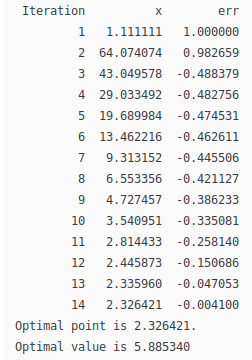
\includegraphics{Newton.png}
    \end{center}
  \part*{2}
    \section*{Code}
      \lstinputlisting[language=python]{SteepestDescent.py}
    \section*{Running}
      \begin{center}
        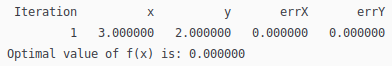
\includegraphics{SteepestDescent.png}
      \end{center}
  \part*{Analysis and Comparation}
    Although both of the 2 methods can help us find the optimal points and values of a function, there are some differences:
    \begin{itemize}
      \item Newton method \\
      This method is originally a root-finding method.\\
      Here we just use Newton method to find the root of the derivative function, which is also the optimal point.\\\\
      \(\Rightarrow\) Therefore, this method is simple in its principle but it is not the best method for optimization. \\
      This can be proved by looking at the \(1^{st}\) problem: a simple \(4^{th}\) degree single variable non-linear function but it requires up to 14 iterations to find out the optimal value.

      \item Steepest descent method \\
      This method, from the result in problem 2, is unarguably faster than Newton method with only 1 iteration needed. \\
      This is due to it being designed to solve optimization problems at first. \\
      However, the main disadvantage of this method that I encounter while applying it is the complexity in its principles. \\
      The first step of finding out the gradient is simple, but the fact that we have to recalculate the value of the gradient in every iteration makes it tedious.\\
      The second step of find out the optimal point in the gradient direction, on the other hand, is a whole root-finding problem of the function's derivative. Thus, it can be very tedious in cases when it is hard to find the derivatives or when the derivative function is hard to solve.\\\\
      \(\Rightarrow\) Therefore, this method is faster, better for optimization but is much more complex and tedious.\\
    \end{itemize}
    
  {\LARGE Conclusion}\\\\
  Newton method is much simpler, thus, it should be prioritized in hand-on calculation with no help from computer.\\\\
  Reversely, steepest descent method should be prioritized as an algorithm in optimization programs because the computer can help us do all the tedious jobs and we can benefit from the advantages of the method. 

\end{document}